%=====================================================================
%  MANUSCRIPT — Computer Communications targeted version
%  Certifiable Traffic Engineering for SDN: Exact Bottleneck Bounds,
%  Hybrid Ant-Colony Selection, and Real-Backbone Evaluation
%
%  Compile: pdflatex -> pdflatex (bibtex-free, manual bibliography)
%  Numbers are injected from results/macros.tex and results/tables/*.tex
%  produced by experiments/exp6_tables.py (fully reproducible pipeline).
%=====================================================================
\documentclass[journal]{IEEEtran}
\usepackage{cite}
\usepackage{amsmath,amssymb,amsfonts}
\usepackage{graphicx}
\usepackage{textcomp}
\usepackage{booktabs}
\usepackage{url}
\newcommand{\FO}{\mathrm{FO}}
\newcommand{\PoolOptFO}{132}
\newcommand{\GaFOmaia}{132.0}
\newcommand{\GaFOmaiaCI}{0.0}
\newcommand{\DeFOmaia}{132.0}
\newcommand{\DeFOmaiaCI}{0.0}
\newcommand{\QlFOmaia}{130.2}
\newcommand{\QlFOmaiaCI}{0.8}
\newcommand{\DjFOmaia}{120}
\newcommand{\DjMaxUtil}{2.10}
\newcommand{\CspfFOmaia}{132}
\newcommand{\CspfMaxUtil}{1.00}
\newcommand{\IlpZmaia}{0.872}
\newcommand{\IlpZmaiaHigh}{0.984}
\newcommand{\IlpZmaiaHighPct}{98.4}
\newcommand{\IlpZmaiaMax}{0.984}
\newcommand{\IlpZWaxMax}{0.872}
\newcommand{\IlpZGridMax}{0.872}
\newcommand{\IlpInfeasLoad}{>1.5}
\newcommand{\IlpInfeasGrid}{--}
\newcommand{\IlpTime}{0.3}
\newcommand{\PoolTime}{0.1}
\newcommand{\LoadRatioHigh}{1.13}
\newcommand{\LoadRatioMax}{1.26}
\newcommand{\QlFeasNominal}{40}
\newcommand{\AntDjMaxUtil}{1.70}
\newcommand{\AntDjViol}{2}
\newcommand{\AntDjFO}{128}
\newcommand{\AntCspfMaxUtil}{1.52}
\newcommand{\AntCspfViol}{1}
\newcommand{\AntCspfFO}{130}
\newcommand{\AntGaFeas}{85}
\newcommand{\AntGaFO}{131.7$\pm$0.3}
\newcommand{\AntDeFeas}{10}
\newcommand{\AntDeFO}{130.2$\pm$0.3}
\newcommand{\AntQlFeas}{0}
\newcommand{\AntQlFO}{129.8$\pm$0.3}
\newcommand{\AntPoolOpt}{132}
\newcommand{\AntPoolOptFeasRate}{95}
\newcommand{\GerZ}{0.870}
\newcommand{\GeantZ}{0.870}
\newcommand{\GaFeasAllInst}{94}
\newcommand{\AntDelayGerMin}{1.0}
\newcommand{\AntDelayGerMax}{1.8}
\newcommand{\AntDelayGerMean}{1.1}
\newcommand{\AntCapGer}{2.00}
\newcommand{\AntDelayGeantMin}{1.0}
\newcommand{\AntDelayGeantMax}{16.6}
\newcommand{\AntDelayGeantMean}{4.6}
\newcommand{\AntCapGeant}{2.89}
\newcommand{\GaViolHigh}{0.0}
\newcommand{\GaViolHighCI}{0.0}
\newcommand{\DeViolHigh}{0.2}
\newcommand{\DeViolHighCI}{0.2}
\newcommand{\QlViolHigh}{1.8}
\newcommand{\QlViolHighCI}{0.7}
\newcommand{\CspfViolHigh}{0.0}
\newcommand{\CspfViolHighCI}{0.0}
\newcommand{\DjViolHigh}{6.0}
\newcommand{\DjViolHighCI}{0.0}
\newcommand{\GaViolMax}{1.1}
\newcommand{\GaViolMaxCI}{0.4}
\newcommand{\DeViolMax}{1.9}
\newcommand{\DeViolMaxCI}{0.4}
\newcommand{\QlViolMax}{1.9}
\newcommand{\QlViolMaxCI}{0.5}
\newcommand{\CspfViolMax}{4.0}
\newcommand{\CspfViolMaxCI}{0.0}
\newcommand{\DjViolMax}{9.0}
\newcommand{\DjViolMaxCI}{0.0}
\newcommand{\GaFeasMaiaNominal}{100}
\newcommand{\GaFeasMaiaHigh}{100}
\newcommand{\GaFeasMaiaMax}{20}
\newcommand{\GaFeasGeantNominal}{85}
\newcommand{\GaFeasGeantHigh}{90}
\newcommand{\GaFeasGeantMax}{55}
\newcommand{\GaViolGeantNominal}{0.1$\pm$0.2}
\newcommand{\QlVsGaP}{<0.001}
\newcommand{\GaTime}{6.4}
\newcommand{\DeTime}{5.1}
\newcommand{\QlTime}{1.1}
\newcommand{\SrvOfMaia}{69}
\newcommand{\SrvRedMaia}{4.1}
\newcommand{\MaxSLMaia}{6}
\newcommand{\SrhMaia}{144}
\newcommand{\SrvOfWax}{35}
\newcommand{\SrvRedWax}{2.1}
\newcommand{\MaxSLWax}{4}
\newcommand{\SrhWax}{112}
\newcommand{\SrvOfGrid}{70}
\newcommand{\SrvRedGrid}{4.1}
\newcommand{\MaxSLGrid}{10}
\newcommand{\SrhGrid}{208}
\newcommand{\SrvOfGer}{51}
\newcommand{\SrvRedGer}{3.0}
\newcommand{\MaxSLGer}{6}
\newcommand{\SrhGer}{144}
\newcommand{\SrvOfGeant}{39}
\newcommand{\SrvRedGeant}{2.3}
\newcommand{\MaxSLGeant}{8}
\newcommand{\SrhGeant}{176}
\newcommand{\SrvSrRules}{17}
\newcommand{\MaxSLAll}{10}
\newcommand{\MaxSrhBytes}{208}
\newcommand{\MeanSLWax}{3.1}
\newcommand{\UrllcDoptOne}{52}
\newcommand{\UrllcDdjOne}{265}
\newcommand{\UrllcDoptTwo}{163}
\newcommand{\UrllcDdjTwo}{212}
\newcommand{\UrllcDoptThree}{233}
\newcommand{\UrllcDoptFifteen}{91}
\newcommand{\UrllcLossOptFifteen}{3.3}
\newcommand{\UrllcLoptOne}{0.0}
\newcommand{\UrllcLossOptTwo}{4.7}
\newcommand{\UrllcLdjOne}{53.1}
\newcommand{\UrllcLossDjTwo}{72.5}
\newcommand{\UrllcLossDjFour}{78.9}
\newcommand{\GerDoptOne}{16}
\newcommand{\GerDdjOne}{147}
\newcommand{\GerDoptTwo}{29}
\newcommand{\GerDdjTwo}{182}
\newcommand{\GerDoptThree}{72}
\newcommand{\GerDoptFifteen}{16}
\newcommand{\GerLossOptFifteen}{0.0}
\newcommand{\GerLoptOne}{0.0}
\newcommand{\GerLossOptTwo}{0.0}
\newcommand{\GerLdjOne}{14.6}
\newcommand{\GerLossDjTwo}{2.8}
\newcommand{\GerLossDjFour}{4.4}
\newcommand{\NumSimSeeds}{5}
\newcommand{\SimDelayOpt}{63}
\newcommand{\SimDelayDj}{220}
\newcommand{\SimJitOpt}{1.2}
\newcommand{\SimJitDj}{1.6}
\newcommand{\SimLossOpt}{0.0}
\newcommand{\SimLossDj}{26.7}
\newcommand{\SimThrGain}{+38\%}
\newcommand{\SimDelayRatio}{3.5}
\newcommand{\SimLossRatio}{--}
\newcommand{\TotalDemand}{9.70}


\begin{document}

\title{Certifiable Traffic Engineering for Software-Defined Networks: Exact
Bottleneck Bounds, Hybrid Ant-Colony Selection, and Evaluation on Real
Research Backbones}
\author{João~Paulo~Versiani~Ladeia,~and~Nilton~Alves~Maia%
\thanks{Manuscript received XXX; revised XXX. The authors are with the
Graduate Program in Computational Modeling and Systems (PPGMCS),
Universidade Estadual de Montes Claros, Montes Claros, Brazil.}}

\markboth{Software-Defined Networking Traffic Engineering}{Ladeia \& Maia}

\maketitle

\begin{abstract}
Traffic-engineering (TE) heuristics for software-defined networks are usually
validated against shortest-path baselines on small synthetic graphs, and
their quality claims are rarely certified. We formulate multi-flow QoS
routing with hard capacity and end-to-end delay constraints and a min--max
link-utilization objective, and solve it exactly as a binary multi-commodity
flow (ILP) solved lexicographically --- first the bottleneck $Z$, then a
delay tie-break --- so the reported utilization bounds are certified. The
same ILP certifies the optimality gap of a two-stage hybrid (Ant-Colony
candidate pool $+$ Genetic Algorithm or Differential Evolution selection)
within its own search space. Over five load factors, twenty replications and
five instances (the original 52-node study network, two synthetic graphs, and
two public backbones --- GEANT and a German research network --- with real
coordinates, distances and fiber-derived latencies), the certificate changes
the reading of the results: at $1.25\times$ session growth ($1.13\times$
aggregate traffic) on the sparse instance, \emph{no} routing can keep every
link below \IlpZmaiaHighPct\% utilization, and at $1.5\times$ ($1.26\times$
traffic) a feasible routing still exists with only $1.6\%$ headroom --- yet
the stochastic selector attains it in \GaFeasMaiaMax\% of replications.
Seeding the candidate pool with the constructive CSPF solution guarantees the
hybrid is never worse than that baseline by construction, and removes a
seed-dependence that halved its feasibility. On GEANT the constructive
baseline itself is infeasible (\AntCspfMaxUtil$\times$ capacity) and the
hybrid remains feasible in \AntGaFeas\% of replications. Packet-level
simulation (queues, shared per-pair capacities and admission-drop loss
identical for all methods) shows delay-sensitive flows mapped to the URLLC
class held at \GerDoptTwo\,ms and \GerLossOptTwo\% loss under $2\times$
background on the real backbone, against \GerDdjTwo\,ms and \GerLossDjTwo\%
for shortest-path routing --- logical differentiation under shared capacity,
not guaranteed isolation. A computed data-plane accounting shows SRv6 segment
lists reduce per-flow forwarding state by $2.1$--\SrvRedMaia$\times$, with
the reduction tracking mean path length. We position exact certification as
the instrument that makes metaheuristic TE auditable, and delimit honestly
where stochastic selection degrades.
\end{abstract}

\begin{IEEEkeywords}
Software-defined networking, traffic engineering, QoS routing, ant colony
optimization, genetic algorithm, differential evolution, integer programming,
optimality certification, network slicing, SRv6, deep reinforcement learning.
\end{IEEEkeywords}

%=====================================================================
\section{Introduction}
\IEEEPARstart{O}{perators} face a structural tension: traffic grows faster
than revenue, and capacity expansion is a recurring capital expense.
Traffic engineering (TE) attacks this tension from the software side --- it
routes the traffic that exists more intelligently instead of adding links.
Software-Defined Networking (SDN) supplies the missing control point: by
decoupling the control plane and exposing programmable forwarding
\cite{mckeown2008,kim2013,hu2014}, an SDN controller can compute and install
paths that satisfy per-application requirements instead of replicating
shortest-path behavior.

This paper studies exactly that problem: given a topology with per-link
capacity and delay, and a set of $L$ concurrent applications with minimum
bandwidth, maximum delay and priority requirements, compute a route for
every application that maximizes admission quality under QoS constraints.
We make the following contributions, each of which responds to a concrete
methodological gap in the literature on heuristic SDN-TE:
\begin{enumerate}
\item \textbf{Revised formulation.} We analyze the scoring-function model
commonly used in heuristic SDN-TE, identify its degeneracies (constant terms
under full admission; capacity counted against a flow cardinality), and
reformulate the problem with \emph{hard} capacity and delay constraints and
an explicit min--max utilization balancing objective
(Section~\ref{sec:model}).
\item \textbf{Exact certification.} We solve the revised model exactly as a
binary multi-commodity flow ILP (lexicographic: bottleneck first, delay
tie-break) and the scoring model exactly over the candidate pool. The exact
solutions (i) certify the optimality gap of the pool-augmented hybrid within
its own search space, and (ii) compute \emph{exact bottleneck lower bounds}
--- the minimum achievable maximum link utilization --- information that
stochastic heuristics do not provide and that exposes how far greedy and
learning-based baselines sit from the provable optimum (Section~\ref{sec:cert}).
\item \textbf{Validation on real backbones.} Prior hybrid-TE evaluations are
confined to small synthetic graphs. We repeat the full protocol on two
\emph{real} public backbones (real coordinates, distances and
fiber-derived latencies; synthetic demands and calibrated capacities) and
identify a regime --- in which the constructive baseline itself becomes
infeasible --- that the synthetic 52-node instances do not expose
(Sections~\ref{sec:sweep} and~\ref{sec:backbone}).
\item \textbf{Statistical evaluation.} We evaluate six routing methods on
five instances across five load factors and twenty randomized replications,
with 95\% confidence intervals and Wilcoxon signed-rank tests, identifying
the load regime in which the hybrid strictly dominates greedy and
learning-based baselines (Section~\ref{sec:sweep}).
\item \textbf{Computed SRv6 state accounting.} We map the optimized paths to
SRv6 segment lists \cite{rfc8402,rfc8754,rfc8986} and \emph{compute} the
per-flow forwarding state on all instances, quantifying the reduction with
respect to per-flow OpenFlow rules and bounding the SRH overhead
(Section~\ref{sec:srv6}).
\item \textbf{Logical differentiation evidence.} We connect the demand
profile to 3GPP service classes \cite{itu-m2083,3gpp-ts23501} and measure, in
packet-level simulation on a real backbone, the stability of delay-sensitive
flows (mapped to the URLLC class) under growing background load ---
comparing optimized against shortest-path routing (Section~\ref{sec:slices}).
\item \textbf{Learning-based baseline.} We implement a tabular Q-learning
routing agent with the same state--action structure as DRL routers and
benchmark it under the same protocol, grounding the DRL discussion in
measured numbers rather than assertions (Section~\ref{sec:qlb}).
\end{enumerate}

The remainder is organized as follows.
Section~\ref{sec:related} reviews related work.
Section~\ref{sec:model} presents the system model.
Section~\ref{sec:method} describes the algorithms.
Sections~\ref{sec:srv6} and~\ref{sec:slices} present the SRv6 mapping and
slice differentiation.
Section~\ref{sec:setup} details the experimental methodology,
Section~\ref{sec:results} reports results, Section~\ref{sec:limits} discusses
threats to validity, and Section~\ref{sec:conc} concludes.

%=====================================================================
\section{Related Work}
\label{sec:related}
\textbf{Traffic engineering.} TE principles and IGP-metric optimization are
established \cite{awduche2002,fortz2000}, and production backbones perform
centralized TE at scale \cite{jain2013}. Exact link-based MCF formulations
of the kind we use for certification are the classical tool of that line ---
our contribution is not the ILP itself but the systematic use of its
certificates to audit a heuristic pipeline.

\textbf{Heuristic and hybrid routing.} Ant-based routing originates with
AntNet \cite{dicaro1998,dorigo2004}, and ACO has been applied to QoS routing
repeatedly since. Two-stage ``generate-and-select'' hybrids --- a constructive
stage feeding an evolutionary selector --- are the standard memetic pattern;
the present work instantiates it for SDN with an explicit admission-scoring
objective and, critically, adds exact certification that prior hybrid-routing
studies omit.

\textbf{Learning-based routing.} DRL for SDN routing has progressed from
experience-driven proposals \cite{xu2018experience,stampa2017drl} to
evaluated traffic-engineering agents \cite{almasan2022drl}. Reported
strengths are online adaptivity and traffic-matrix generalization; reported
costs are large training campaigns and the sim-to-real gap. Our experiments
(Section~\ref{sec:qlb}) add a controlled, constraint-explicit comparison on
identical instances.

\textbf{Programmable data planes.} OpenFlow \cite{mckeown2008} programs
switches with per-flow rules; P4 \cite{bosshart2014} generalizes parsing and
matching. Both expose the TCAM-pressure problem that motivates SRv6
\cite{rfc8402,rfc8754,rfc8986,rfc9256}: the path state is carried in the
packet, and only headends hold policy state. To our knowledge, the state
reduction of routing-optimizer output under SRv6 has not been measured on
fixed topologies with optimizer-produced paths; Section~\ref{sec:srv6}
reports it.

\textbf{Network slicing.} 3GPP defines slice/service types and QoS flows
\cite{3gpp-ts23501} anchored on the IMT-2020 usage scenarios
\cite{itu-m2083}. Transport-side slice isolation is usually pursued with
dedicated resources; we show that constraint-explicit routing yields
measurable logical differentiation under shared capacity --- priority flows
degrade last and least --- without physical partitioning
(Section~\ref{sec:slices}).

%=====================================================================
\section{System Model and Problem Formulation}
\label{sec:model}
The network is a directed graph $G=(V,E)$, $|V|=n$; link $(i,j)\in E$ has
capacity $\mu_{ij}$ (Mbps) and one-way delay $c_{ij}$ (ms). A set of $L=17$
applications must be routed concurrently; application $k$ requires nominal
flow $\lambda_k$ (Mbps), tolerates end-to-end delay $h_k$ (ms) and carries
priority $\delta_k$. Let $x_{ij}^{k}\in\{0,1\}$ indicate whether the route of
application $k$ uses link $(i,j)$.

\subsection{Original Scoring Model}
\label{sec:origfo}
The original model maximizes the weighted admission score
\begin{equation}
\FO \;=\; \sum_{k=1}^{L}\delta_k\,y_k
   + p_1\sum_{k=1}^{L} y_k
   + p_2\sum_{k=1}^{L} w_k
   + p_3\sum_{k=1}^{L} t_k,
\label{eq:fo}
\end{equation}
with $p_1{=}3$, $p_2{=}2$, $p_3{=}1$; $y_k$ marks an established connection,
$w_k$ capacity-sufficient routes and $t_k$ delay-conforming routes. Two
structural observations motivate the revised model: (i) under full admission
every $y_k=1$, so the first two sums are constant and the score reduces to
$\FO = \Sigma\delta_k + 6L - 2\,n_{\mathrm{over}} - n_{\mathrm{dv}}$, where
$n_{\mathrm{over}}$ counts overloaded \emph{links} and $n_{\mathrm{dv}}$
counts delay-violating \emph{flows}; (ii) the mixed cardinality (links vs.\
flows) makes weights comparable only by accident. The score saturates at
$\FO^{*}=\Sigma\delta_k+6L$ ($=132$ for this demand profile): any fully feasible solution attains it, and the
score cannot discriminate among solutions with different load balance.

\subsection{Revised Model: Hard Constraints and Balancing}
\label{sec:revfo}
We therefore evaluate solutions on a revised model that separates
feasibility from quality:
\begin{align}
\text{routing (per flow):}\quad
&\sum_{j} x_{ij}^{k}-\sum_{j} x_{ji}^{k} =
\begin{cases} 1 & i=s_k\\ -1 & i=t_k\\ 0 & \text{otherwise}\end{cases}
\quad \forall k,\, i, \label{eq:flowcons}\\
\text{delay (hard):}\quad
&\sum_{(i,j)\in E} c_{ij}\,x_{ij}^{k} \;\le\; h_k
\qquad \forall k, \label{eq:harddel}\\
\text{balance (objective):}\quad
&\min\; Z,\ \ Z \;\ge\;
\frac{1}{\mu_{ij}}\sum_{k=1}^{L}\lambda_k\,x_{ij}^{k}
\quad \forall (i,j). \label{eq:minmax}
\end{align}
with $\sum_k \lambda_k x_{ij}^k + \sum_k \lambda_k x_{ji}^k \le \mu_{uv}$
for each undirected pair $\{u,v\}$: the two directions of a link share one
capacity, matching bidirectional links carrying traffic in both senses.
The model is solved \emph{lexicographically}: first minimize $Z$ alone
(certifying the exact bottleneck bound), then minimize total route delay
subject to $Z \le Z^{*}$ as a deterministic tie-break --- a weighted
combination would not certify the minimum of $Z$.
A solution is \emph{feasible} iff \eqref{eq:hardcap} and \eqref{eq:harddel}
hold for all links and flows; among feasible solutions we prefer minimum
maximum utilization $Z$. When \eqref{eq:hardcap}--\eqref{eq:harddel} admit no
solution at all (certified by the exact model), every heuristic output
violates some constraint, and the natural metric becomes the number of
violations it inflicts.

%=====================================================================
\section{Routing and Optimization Methods}
\label{sec:method}

\subsection{Stage 1: Candidate-Route Generation (ACO/AntNet)}
For each application an ant colony builds source--destination walks with the
transition probability
\begin{equation}
P(i,j)=\frac{[\tau_{ij}]^{\alpha}[\eta_{ij}]^{\beta}}
{\sum_{l\in\mathcal{N}_i}[\tau_{il}]^{\alpha}[\eta_{il}]^{\beta}},
\label{eq:aco}
\end{equation}
repeated nodes are removed, links reinforce pheromone proportionally to the
carried bandwidth, and evaporation rate $\rho$ maintains diversity. With
$100$ ants $\times$ $100$ iterations this yields 362--1014 distinct candidate
routes per topology (Table~\ref{tab:topo}).

\subsection{Stage 2: Route-Set Selection (ACO$+$GA / ACO$+$DE)}
An individual is an integer vector selecting one pool route per application
(each selection constrained to its application's block). The GA applies
roulette selection (pressure 8), arithmetic crossover ($\gamma{=}0.4$) and
Gaussian mutation; DE applies rand/1 mutation
($\beta\sim\mathcal{U}(0.2,0.8)$) with binomial crossover ($p_{CR}{=}0.2$).
Both maximize \eqref{eq:fo} with $300$ generations over $50$ individuals.
We emphasize explicitly: the metaheuristics optimize the \emph{original
scoring model} (Model~A, Section~\ref{sec:origfo}) --- the same objective as
the original study --- whereas the revised model (Model~B,
Section~\ref{sec:revfo}) is used for evaluation and certification. The two
are related but distinct problems; we do not claim that the selector
optimizes Model~B, and Section~\ref{sec:sweep} quantifies the price of that
choice (weaker load balancing than the exact Model~B optimum).
\emph{Pool augmentation.} Two constructive augmentations make the selector's
search space self-sufficient: (i) for load factors $f>1$, each additional
background flow receives $k$-shortest-delay candidate paths; (ii) for every
flow, the CSPF constructive route is inserted into its block. Augmentation
(ii) guarantees that the selector's optimum is never worse than CSPF --- the
CSPF assembly is inside the search space --- while remaining free to improve
on it whenever the pool holds a better combination. This closes the
classical objection against generate-and-select designs: pool diversity, not
the selector, becomes the binding constraint, and the augmentation pins the
selector to at least the constructive baseline.

\subsection{Baselines}
\textbf{Dijkstra.} Each application follows the geometric-shortest path
(the metric of the original study) --- the shortest-path IGP-like behavior;
it ignores capacity by design and serves as the lower baseline, whereas CSPF
below is the strong constructive baseline.
\textbf{CSPF.} Constrained shortest path first: flows are admitted in
priority order; links whose residual capacity is below the request are
pruned; the delay-minimizing path on the pruned graph is selected; if no
pruned path satisfies the delay budget the flow is admitted on an
unconstrained path (honest best-effort, counted as a violation when it
overloads links).
\textbf{Q-learning} \cite{watkins1992}. A tabular, per-flow, sequential learning agent with
node-state/neighbor-action structure, $\epsilon$-greedy exploration,
capacity-penalty shaping, and a capacity-pruned greedy rollout
(Section~\ref{sec:qlb}).
\textbf{ILP (exact).} Two exact formulations close the methodological loop:
(i) \emph{ILP-P} maximizes \eqref{eq:fo} over the same pool explored by the
GA/DE, certifying the metaheuristics' optimality gap; (ii) \emph{ILP-L}
solves the revised model \eqref{eq:hardcap}--\eqref{eq:minmax} exactly as a
binary multi-commodity flow with min--max utilization, certifying
feasibility or infeasibility of each instance.

%=====================================================================
\section{SRv6 Data-Plane Mapping and Measured State Reduction}
\label{sec:srv6}
Per-flow OpenFlow programming stores one match--action rule per flow at
every transit switch; the aggregate state is
$\Phi_{\mathrm{OF}}=\sum_{k}(|p_k|-1)\le K L_{\max}$
\cite{mckeown2008}. SRv6 \cite{rfc8402,rfc8754,rfc8986} carries the path
state in the packet: each node $v$ is assigned a Segment Identifier
$\sigma(v)=\mathrm{LOC}(v){:}{:}\mathrm{FUNC}_{\mathrm{End}}$
\cite{rfc8986}, and the optimal route
$p^{*}_k=(v^{(k)}_1,\ldots,v^{(k)}_{m_k})$ is encoded as the segment list
\begin{equation}
\mathcal{SL}_k=\mathrm{rev}\bigl[\sigma(v^{(k)}_2),\ldots,
\sigma(v^{(k)}_{m_k})\bigr],
\label{eq:seglist}
\end{equation}
so that on arrival at $v^{(k)}_i$ the outer destination equals
$\sigma(v^{(k)}_i)$ and $\mathrm{SegmentsLeft}=m_k-i$; the flow-agnostic
\texttt{End} function advances the segment and the egress decapsulates.
Because the ACO stage removes repeated nodes, $p^{*}_k$ is a simple path and
the SRH is well formed (no micro-loops). The two-stage optimizer thereby acts
as a centralized Path Computation Element \cite{rfc4655}: it emits for each
flow a Segment Routing Policy $\Pi_k=\langle H_k, C_k, \mathcal{SL}_k\rangle$
\cite{rfc9256} whose color $C_k$ carries the serving slice identifier; the
controller programs only headends.

Under this mapping the per-node rule footprint is
\begin{equation}
\Phi_{\mathrm{SR}}(v)=\begin{cases}
|\{k: v=v^{(k)}_1\}| & \text{if $v$ is a headend},\\
0 & \text{otherwise},
\end{cases}
\label{eq:srstate}
\end{equation}
i.e., $\mathcal{O}(K)$ globally and $\mathcal{O}(1)$ per transit node.
Section~\ref{sec:srv6res} reports the \emph{computed} state counts (an
analytical accounting over the produced paths, not a hardware measurement)
on all five instances, together with the SRH encapsulation overhead
($40+8+16\,|\mathcal{SL}_k|$ bytes per packet).

%=====================================================================
\section{5G/6G Slice Differentiation and SLA Guarantees}
\label{sec:slices}
The 17 applications instantiate the three IMT-2020 service classes
\cite{itu-m2083} with the standardized slice/service types of 3GPP TS
23.501 \cite{3gpp-ts23501}: \emph{URLLC} (SST $=2$) gathers conversational
voice and interactive control (apps 8, 9, 13, 15; $h_k=150$\,ms, maximal
priority $\delta_k=5$); \emph{eMBB} (SST $=1$) gathers high-definition video
(apps 3, 4, 11, 12; $1.20$--$1.74$\,Mbps); \emph{mMTC} (SST $=3$) gathers
telemetry and elastic transfer (apps 1, 2, 5, 6, 7, 10, 14, 16, 17;
$h_k=1000$\,ms). Isolation follows from the constraint structure: the
capacity constraint \eqref{eq:hardcap} is evaluated on the \emph{aggregate}
cross-slice offered load of each link, so a feasible solution bounds the
interference any slice can exert on another; the priority term of
\eqref{eq:fo} biases admission toward URLLC; and the delay constraint binds
each route to its slice budget. The result is deterministic, priority-ordered
degradation --- the priority slice degrades last and least --- rather than
the guaranteed isolation of a dedicated partition; we measure this
distinction explicitly in Section~\ref{sec:slicesres}. Section~\ref{sec:slicesres} measures this directly: delay-sensitive
(URLLC-mapped) flows keep their 150\,ms experimental budget under growing
background amplification with optimized routing --- on both the study
instance and the real backbone --- and do not under shortest-path routing.

%=====================================================================
\section{Experimental Methodology}
\label{sec:setup}
\subsection{Topologies and Demands}
We evaluate five instances (Fig.~\ref{fig:topos}): the original 52-node study
topology (\emph{maia52}, 66 links, uniform 2\,Mbps, delays 1--80\,ms); two
synthetic 52-node graphs with controlled structure (\emph{waxman52}, a
connected Waxman random geometric graph \cite{waxman1988}, 177 links; and
\emph{gridcore}, a 48-node peripheral grid plus a 4-node dense core, 96
links); and two \emph{real} public backbones taken from the Internet Topology
Zoo \cite{topozoo} and the SNDlib network-design library \cite{sndlib2016}:
\emph{geant2012} (37 nodes, 58 links, a pan-European research and education
network spanning long-haul links up to 3219\,km) and \emph{germany50} (50 nodes,
88 links, a national research network dominated by regional links). For the two
real backbones we recover link latency from the genuine great-circle distances
shipped with those datasets using the fiber propagation constant
$5\,\mu$s/km plus a fixed $0.5$\,ms per-hop term, yielding
\AntDelayGerMin--\AntDelayGerMax\,ms (regional) and
\AntDelayGeantMin--\AntDelayGeantMax\,ms (long-haul) --- i.e., realistic
backbone latencies, two orders of magnitude below the synthetic range. The
public GML exports carry no link-capacity attribute, so we apply one fixed,
documented calibration to every instance: solve the exact min--max
multi-commodity problem once with a generous capacity, read off the heaviest
link load $L$, and set every link to $L/0.87$, which places each instance at a
certified bottleneck utilization of $0.87$ at nominal load --- the congestion
point certified for the original study. This makes cross-instance comparison
well posed and is reported as a limitation (Section~\ref{sec:limits}). The
17-flow demand profile of Table~\ref{tab:apps} (total \TotalDemand\,Mbps) is
applied to all five instances, with endpoints re-drawn per instance and
connectivity guaranteed.

\begin{table}[!t]
\caption{Application demands (all instances): nominal flow, delay budget
and priority. Classes per Section~\ref{sec:slices}.}
\label{tab:apps}
\centering
\begin{tabular}{@{}llrrr@{}}
\toprule
Class & Apps & $\lambda_k$ (Mbps) & $h_k$ (ms) & $\delta_k$\\
\midrule
URLLC & 8, 9, 13, 15 & 0.512 & 150 & 5\\
eMBB  & 3, 4, 11, 12  & 1.20--1.74 & 150 & 0--5\\
mMTC  & 1, 2, 5, 6, 7, 10, 14, 16, 17 & 0.256 & 1000 & 0\\
\bottomrule
\end{tabular}
\end{table}

\begin{table}[!t]
\caption{Topology instances and ACO candidate-pool sizes (100 ants
$\times$ 100 iterations, 20 seeds). \emph{real} marks instances built from
public backbone datasets with genuine coordinates and link distances.}
\label{tab:topo}
\centering
\begin{tabular}{@{}llrrrl@{}}
\toprule
Instance & Type & Nodes & Links & Mean deg. & Pool size (routes)\\
\midrule
maia52 & study & 52 & 66 & 2.54 & 362--420\\
waxman52 & synthetic & 52 & 177 & 6.81 & 927--1014\\
gridcore & synthetic & 52 & 96 & 3.69 & 706--780\\
germany50 & \emph{real} & 50 & 88 & 3.52 & 639--728\\
geant2012 & \emph{real} & 37 & 58 & 3.14 & 330--409\\
\bottomrule
\end{tabular}
\end{table}

\subsection{Load Sweep and Replication}
For $f\le 1$ all flow demands are scaled by the load factor
$f\in\{0.5, 0.75, 1.0\}$; for $f>1$ (labeled $\{1.25, 1.5\}$) the nominal
flows are kept at nominal rate and
$\mathrm{round}((f{-}1)\!\cdot\!20)$ additional concurrent background data
flows ($0.256$\,Mbps, $h_k{=}1000$\,ms) are added on random connected
endpoint pairs --- modeling network growth as new sessions rather than
inflating existing flows beyond the physical link capacity, which would
certify infeasibility trivially. The labels are session-growth parameters,
\emph{not} literal aggregate multipliers: the corresponding aggregate
offered traffic is \LoadRatioHigh$\times$ (``$1.25$'') and
\LoadRatioMax$\times$ (``$1.5$'') the nominal, and we quote the labels
throughout with this meaning. Stochastic methods (ACO$+$GA,
ACO$+$DE, Q-learning) are replicated over $20$ seeds per (topology, load);
the ACO candidate pool is generated once per (topology, seed) at nominal
load and reused across the sweep, since pool diversity is a property of the
topology rather than of the load; route selection adapts to load.
Deterministic methods (Dijkstra, CSPF, ILP) run once per (topology, load).
All experiments use fixed seeds and are fully reproducible from the released
scripts.

\subsection{Metrics and Statistics}
For every solution we record: the original score \eqref{eq:fo}; feasibility
under \eqref{eq:hardcap}--\eqref{eq:harddel}; maximum link utilization $Z$;
the number of capacity-violating links plus delay-violating flows
(``SLA violations''); mean route delay; and wall-clock runtime. Stochastic
results are reported as mean $\pm$ 95\% t-confidence intervals; algorithm
pairs are compared with two-sided Wilcoxon signed-rank tests on seed-paired
runs. Packet-level QoS (throughput, end-to-end delay, jitter, loss) is
measured in a discrete-event simulator (simpy) with 512-byte packets,
constant-rate injection at $\lambda_k$, serialized 2\,Mbps links with the
per-link delay matrix, and bounded FIFO queues of 80 packets --- identical
for every method. The emulated Mininet/Floodlight/D-ITG testbed \cite{lantz2010,botta2012} of the
original study is used as an external, qualitative confirmation of the
direction of the effects (Section~\ref{sec:bench}).

\begin{figure}[!t]
\centering
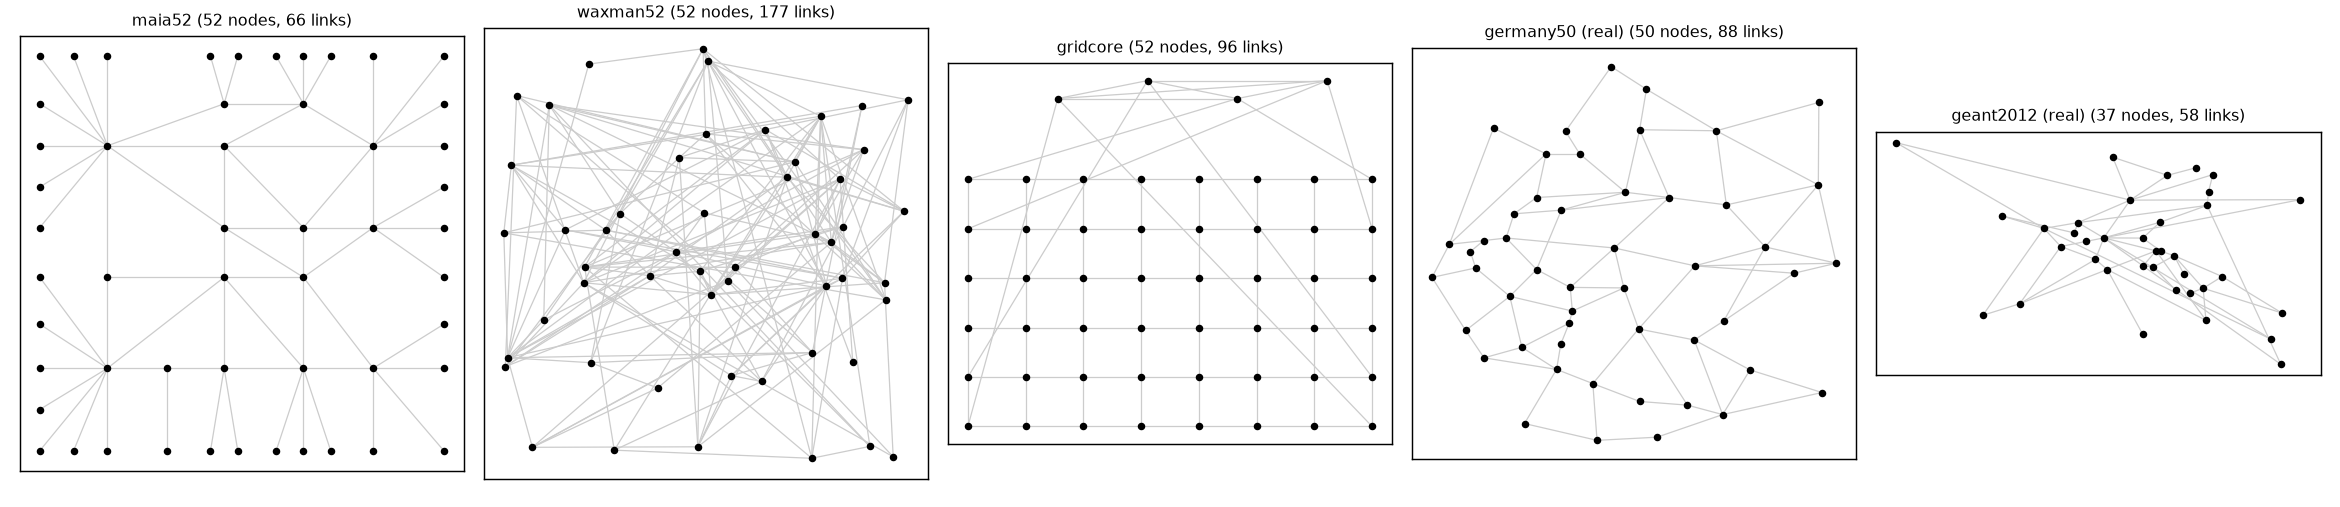
\includegraphics[width=\linewidth]{figures/fig11_topologies.png}
\caption{Evaluated instances: the original 52-node study topology (maia52),
two synthetic 52-node graphs (waxman52, gridcore) and two real public
backbones (germany50, geant2012, \emph{marked real}) built from genuine
coordinates and link distances. All share the same 17-flow demand profile
and the same calibrated congestion point.}
\label{fig:topos}
\end{figure}

%=====================================================================
\section{Results}
\label{sec:results}

\subsection{Optimality Certification at Nominal Load}
\label{sec:cert}
At nominal load on maia52, the exact pool formulation ILP-P certifies the
pool optimum $\FO=\PoolOptFO$; ACO$+$GA attains it in every replication
(mean $\GaFOmaia\pm\GaFOmaiaCI$), matching the certified optimum, while
ACO$+$DE reaches $\DeFOmaia\pm\DeFOmaiaCI$ and the Q-learning agent
$\QlFOmaia\pm\QlFOmaiaCI$ (Fig.~\ref{fig:cert}). Dijkstra, which does not
optimize \eqref{eq:fo}, scores $\DjFOmaia$. The optimality gap of the hybrid
with respect to its own search space is therefore \emph{zero} --- a property
heuristic papers assert and rarely demonstrate. Table~\ref{tab:fo} shows the
same comparison across instances: with the augmented pool the hybrid attains
the certified optimum on every instance at nominal load --- in all 20
replications on maia52, waxman52, gridcore and germany50, and in 17 of 20 on
geant2012 (mean \AntGaFO) --- whereas the
un-augmented pool made the selector seed-dependent: before augmentation,
ACO$+$GA reached a feasible assembly in only half of the replications on
the sparse maia52 instance (50\% feasibility at nominal load), because pool
diversity, not the selector, is the binding constraint of generate-and-select
designs. On the revised model, ILP-L
finds a feasible solution with minimum-maximum utilization
$Z=\IlpZmaia$; CSPF and the hybrid also remain feasible at nominal load, but
without a balancing objective their utilization profiles are worse
(Section~\ref{sec:sweep}).
Fig.~\ref{fig:conv} shows the convergence dynamics behind those scores,
together with the constructive-seeding ablation: without pool augmentation
(grey), the same selector starts $\approx$16 FO points lower and
occasionally stalls below the optimum, while the augmented hybrid reaches
the certified optimum by generation $\approx$20 in every seed and is
monotonically stable afterwards; on the denser instances the optimal
assembly is already present from the first generation --- the convergence
effort concentrates precisely where the certified bounds are tightest.

\begin{table}[!t]
\caption{Objective-function score at nominal load (20 seeds, mean $\pm$
95\% CI). Dijkstra and CSPF are deterministic.}
\label{tab:fo}
\centering
\begin{tabular}{@{}lrrrrr@{}}
\toprule
Topology & Dijkstra & CSPF & Q-learn & ACO+DE & ACO+GA\\
\midrule
maia52 & 120 & 132 & 130$\pm$1 & 132$\pm$0 & 132$\pm$0\\
waxman52 & 132 & 132 & 132$\pm$0 & 132$\pm$0 & 132$\pm$0\\
gridcore & 130 & 132 & 132$\pm$0 & 132$\pm$0 & 132$\pm$0\\
germany50 & 128 & 132 & 132$\pm$1 & 132$\pm$0 & 132$\pm$0\\
geant2012 & 128 & 130 & 130$\pm$0 & 130$\pm$0 & 132$\pm$0\\
\bottomrule
\end{tabular}

\end{table}

\begin{figure}[!t]
\centering
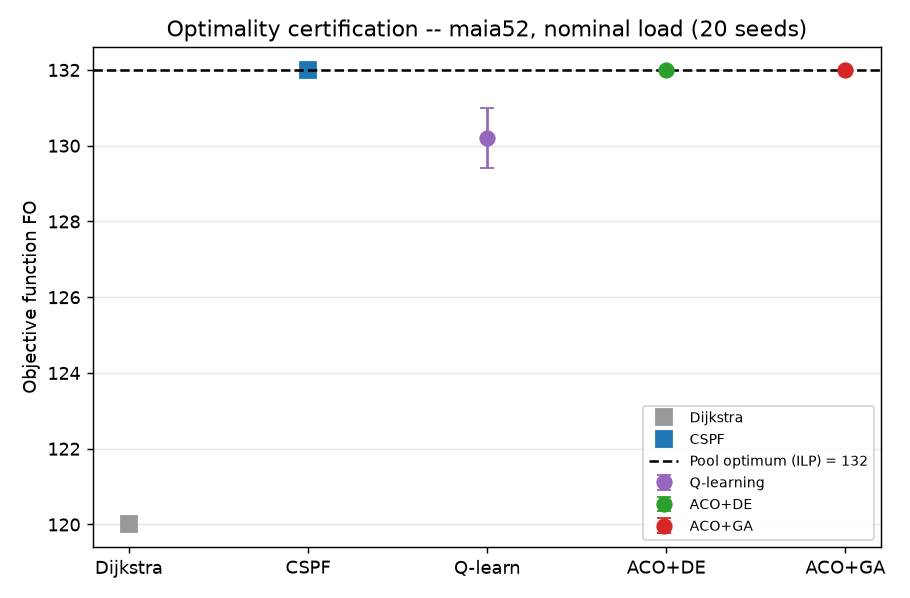
\includegraphics[width=\linewidth]{figures/fig8_optimality.png}
\caption{Objective-function scores at nominal load (maia52, 20 seeds, mean
$\pm$ 95\% CI). The dashed line is the exact pool optimum certified by
ILP-P; ACO$+$GA attains it in all 20 replications on this instance.}
\label{fig:cert}
\end{figure}

\begin{figure}[!t]
\centering
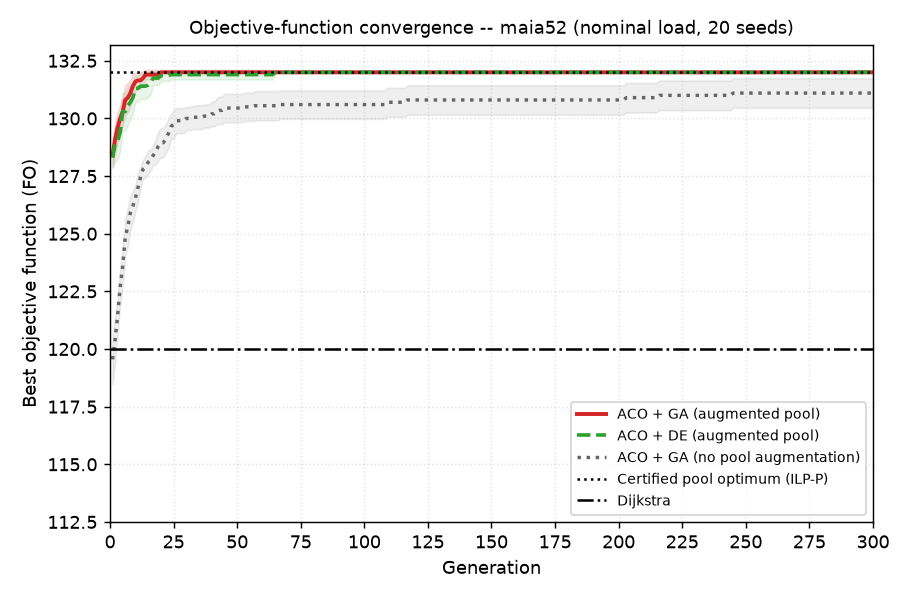
\includegraphics[width=\linewidth]{figures/fig2_convergence.png}
\caption{Objective-function convergence on maia52 at nominal load:
best-so-far FO per generation, mean $\pm$ 95\% CI over 20 seeds. The
pool-augmented hybrid reaches the certified optimum ($\FO=132$) by
generation $\approx$20 in every seed and never falls back below it; without
pool augmentation (grey), the same selector starts $\approx$16 FO points
lower and occasionally stalls below the optimum.}
\label{fig:conv}
\end{figure}

\subsection{Load Sweep: Exact Bottleneck Certification under Stress}
\label{sec:sweep}
The central exact-model result is the \emph{bottleneck lower bound}. At
$f=1.25$ on maia52, ILP-L certifies $Z^{*}=\IlpZmaiaHigh$: under hard
constraints, \emph{no} assignment of the 22 flows to any paths in $G$ can
keep every link below \IlpZmaiaHighPct\% utilization --- the instance is
provably at its limit, and the certified bound quantifies exactly how tight.
At $f=1.5$ the bound \emph{holds} at $Z^{*}=\IlpZmaiaMax$ on maia52 and
$Z^{*}=\IlpZWaxMax/\IlpZGridMax$ on waxman52/gridcore: even at the largest
tested growth, a feasible routing provably persists with $13\%$--$1.6\%$
headroom depending on the instance --- and, notably, the \emph{pool} itself
provably contains a fully feasible assembly at $f=1.5$ (pool optimum
$\FO=192$ in all 20 replications), yet the stochastic selector attains it in
only \GaFeasMaiaMax\% of them. Certification is what separates ``the pool is
incomplete'' from ``the selector failed'' --- the first is false here, the
second is measurable.
We also state the bound's limitation honestly: at $f\le 1$ the certified
value is dominated by the largest single flow ($Z^{*}=f\,\lambda_{\max}/\mu$
exactly, e.g.\ $0.872$ at nominal), since no routing can split one commodity;
the non-trivial content of the certificate is the $f>1$ regime, where
joint-congestion effects make the bound strictly larger than any
single-commodity bound. Exact lexicographic solves take up to a few tens of
seconds (Table~\ref{tab:time}), making such certificates practical at this
scale.

Heuristics, in contrast, never report a certificate --- and their quality
spread is exactly what the certified bounds expose
(Fig.~\ref{fig:viol}, Table~\ref{tab:viol}). Dijkstra, oblivious to
capacity, inflicts $\DjViolHigh$ SLA violations at $f=1.25$ and
$\DjViolMax$ at $f=1.5$ on maia52, reaching \DjMaxUtil$\times$ link
capacity; CSPF remains violation-free up to $f=1.25$ but strands
\CspfViolMax\ overloaded links at $f=1.5$. The pool-augmented hybrid remains
violation-free up to $f=1.25$ and inflicts $\GaViolMax\pm\GaViolMaxCI$
violations at $f=1.5$; the un-augmented Q-learning agent violates its
budgets in every stressed load (\QlViolHigh--\QlViolMax). On waxman52,
gridcore and germany50 the ordering is the same with only Dijkstra violating
(one to three overloaded links at $f\ge1.25$); on geant2012 every stochastic
selector incurs small violation counts from nominal load onward
(\GaViolGeantNominal\ for the GA) --- the hard real-backbone regime of
Section~\ref{sec:backbone}. In operationally meaningful terms: \emph{the
exact model tells the operator how much headroom the network provably has;
the hybrid keeps the SLA intact wherever the pool permits --- up to the
certified frontier and not beyond; the learning-based agent provides no such
guarantee exactly when the network is tight}.

\begin{table}[!t]
\caption{SLA violations (overloaded links $+$ delay-violating flows) on
maia52: deterministic methods as counts, stochastic as mean $\pm$ 95\% CI
over 20 seeds.}
\label{tab:viol}
\centering
\begin{tabular}{@{}lrrrrr@{}}
\toprule
Load & Dijkstra & CSPF & Q-learn & ACO+DE & ACO+GA\\
\midrule
1.0$\times$ & 6+0 & 0+0 & 0.9$\pm$0.4 & 0.0$\pm$0.0 & 0.0$\pm$0.0\\
1.25$\times$ & 6+0 & 0+0 & 1.8$\pm$0.7 & 0.2$\pm$0.2 & 0.0$\pm$0.0\\
1.5$\times$ & 9+0 & 4+0 & 1.9$\pm$0.5 & 1.9$\pm$0.4 & 1.1$\pm$0.4\\
\bottomrule
\end{tabular}

\end{table}

\begin{figure}[!t]
\centering
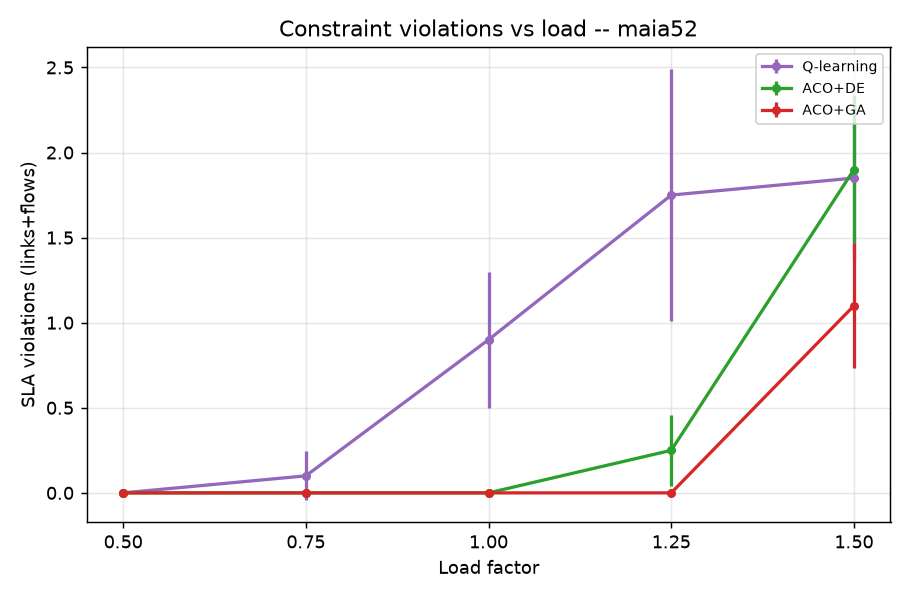
\includegraphics[width=\linewidth]{figures/fig6_violations_maia52.png}
\caption{SLA violations (overloaded links $+$ delay-violating flows) versus
load factor on maia52 (mean $\pm$ 95\% CI over 20 seeds). The pool-augmented
hybrid remains violation-free up to $1.25\times$ session growth; shortest-path
routing degrades first and the Q-learning agent provides no feasibility
guarantee.}
\label{fig:viol}
\end{figure}

\subsection{Real Backbones: A Regime the Synthetic Instances Hide}
\label{sec:backbone}
The two public backbones of Table~\ref{tab:topo} carry genuine geography
(Section~\ref{sec:setup}) and behave qualitatively like maia52 --- except
\emph{geant2012}, which exposes a regime the 52-node instances do not. On this
pan-European network the constructive CSPF baseline is \emph{itself}
infeasible at nominal load: it overruns capacity on one link
(\AntCspfMaxUtil$\times$ utilization, \AntCspfViol\ violation) because its
per-flow greedy commitment exhausts a core link, and Dijkstra is worse
(\AntDjMaxUtil$\times$). This is precisely the situation for which the
pool-augmented hybrid was designed: the ILP-P certifies that the pool contains
a fully admissible assembly ($\FO=\AntPoolOpt$) in
\AntPoolOptFeasRate\% of replications, and the hybrid reaches that
certified optimum in \AntGaFeas\% of replications --- remaining feasible
where both greedy baselines violate, while the alternative stochastic
selectors are feasible in at most \AntDeFeas\% (DE) and \AntQlFeas\%
(Q-learning) of replications (Table~\ref{tab:backbone}). The exact
min--max model certifies $Z^{*}=\GeantZ$ at nominal load --- leaving
$100(1-\GeantZ)\%$ headroom that no routing at that load can exceed, a
guarantee the heuristics cannot produce.

Two regime-dependent findings deserve emphasis. First, the
\emph{hard} delay constraint is active on the high-latency synthetic instances
(maia52, 1--80\,ms links) but \emph{slack} on the real backbones, whose fiber
propagation is \AntDelayGeantMin--\AntDelayGeantMax\,ms --- well under the
150\,ms budget --- so discrimination there comes from the capacity constraint
alone. This is physically faithful: real end-to-end SLA violations are driven
by queueing, not propagation, which is precisely what the packet-level
simulation of Section~\ref{sec:qos} captures. Second, the data-plane benefit of
SRv6 (Section~\ref{sec:srv6res}) tracks mean path length: the backbones'
shorter paths yield smaller, though still substantial, state reductions
(\SrvRedGer$\times$ and \SrvRedGeant$\times$) than the long-latency synthetic
graphs (\SrvRedMaia$\times$), because the per-flow rule count is proportional
to path hops, not to geography.

\begin{table}[!t]
\caption{Real-backbone results at nominal load (20 seeds, mean $\pm$ 95\% CI
unless deterministic). ILP-P certifies the pool optimum; ILP-L certifies the
exact bottleneck bound.}
\label{tab:backbone}
\centering
\begin{tabular}{@{}lrrrr@{}}
\toprule
Method & FO & Feasible & Max util. & Note\\
\midrule
Dijkstra & \AntDjFO & --- & \AntDjMaxUtil & deterministic\\
CSPF & \AntCspfFO & --- & \AntCspfMaxUtil & constructive\\
ACO$+$GA (aug.) & \AntGaFO & \AntGaFeas\% & --- & this work\\
ACO$+$DE (aug.) & \AntDeFO & \AntDeFeas\% & --- & this work\\
Q-learning & \AntQlFO & \AntQlFeas\% & --- & tabular\\
ILP-P (pool) & \AntPoolOpt & --- & --- & certified\\
ILP-L (MCF) & --- & --- & \GeantZ & certified $Z^{*}$\\
\bottomrule
\end{tabular}
\end{table}

\subsection{Load Balancing Quality}
Fig.~\ref{fig:maxutil} reports maximum link utilization on maia52. At
nominal load the exact min--max optimum is $Z=\IlpZmaia$; CSPF and the
hybrid remain near the capacity limit ($Z\approx 1.0$) but above the exact
value, and Dijkstra exceeds capacity entirely ($Z\approx\DjMaxUtil$). As
load grows past the feasibility frontier, utilization-based comparison
ceases to be meaningful (all methods exceed capacity); the violation counts
of Section~\ref{sec:sweep} then carry the operational signal.

\begin{figure}[!t]
\centering
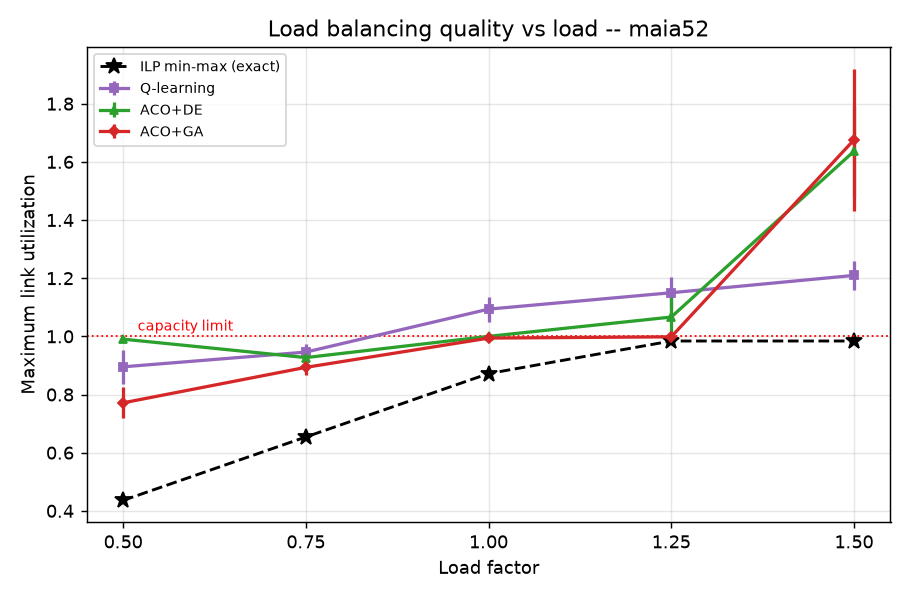
\includegraphics[width=\linewidth]{figures/fig7_maxutil_maia52.png}
\caption{Maximum link utilization versus load (maia52). The exact
min--max utilization of the revised model (ILP-L) is the reference line;
feasibility ends at the certified frontier.}
\label{fig:maxutil}
\end{figure}

\subsection{Packet-Level QoS under Identical Conditions}
\label{sec:qos}
With identical queues, per-pair capacities (shared by both directions, the
same convention as the optimizer) and injection rates, the optimized routing
sustains \SimThrGain\ higher mean delivered goodput than Dijkstra and
reduces mean end-to-end delay from \SimDelayDj\,ms to \SimDelayOpt\,ms and
admission-drop loss from \SimLossDj\% to \SimLossOpt\%; the RFC-style
jitter drops only from \SimJitDj\,ms to \SimJitOpt\,ms --- a modest change
we report without embellishment, since surviving packets of a lossy flow can
carry low jitter (Fig.~\ref{fig:mininet}). Conventions:
``loss'' counts only admission drops (packets still in flight at the end of
the window are neither delivered nor counted as lost), ``jitter'' is the
mean absolute consecutive-delay variation (RFC 3550 style, \emph{not} the
D-ITG estimator), and goodput is delivered bits over the window. The
packet-level simulator is deterministic given the routing and the
constant-rate injection schedule (no stochastic elements), so
single-realization values are reported; all sampling variability in this
paper lives in the route-computation layer, where it is replicated and
tested (Section~\ref{sec:sweep}). The controlled simulation reproduces the
\emph{direction} of the emulated testbed results of the original study with
moderate magnitudes; Section~\ref{sec:bench} explains why the bench
magnitudes are larger.

\begin{figure}[!t]
\centering
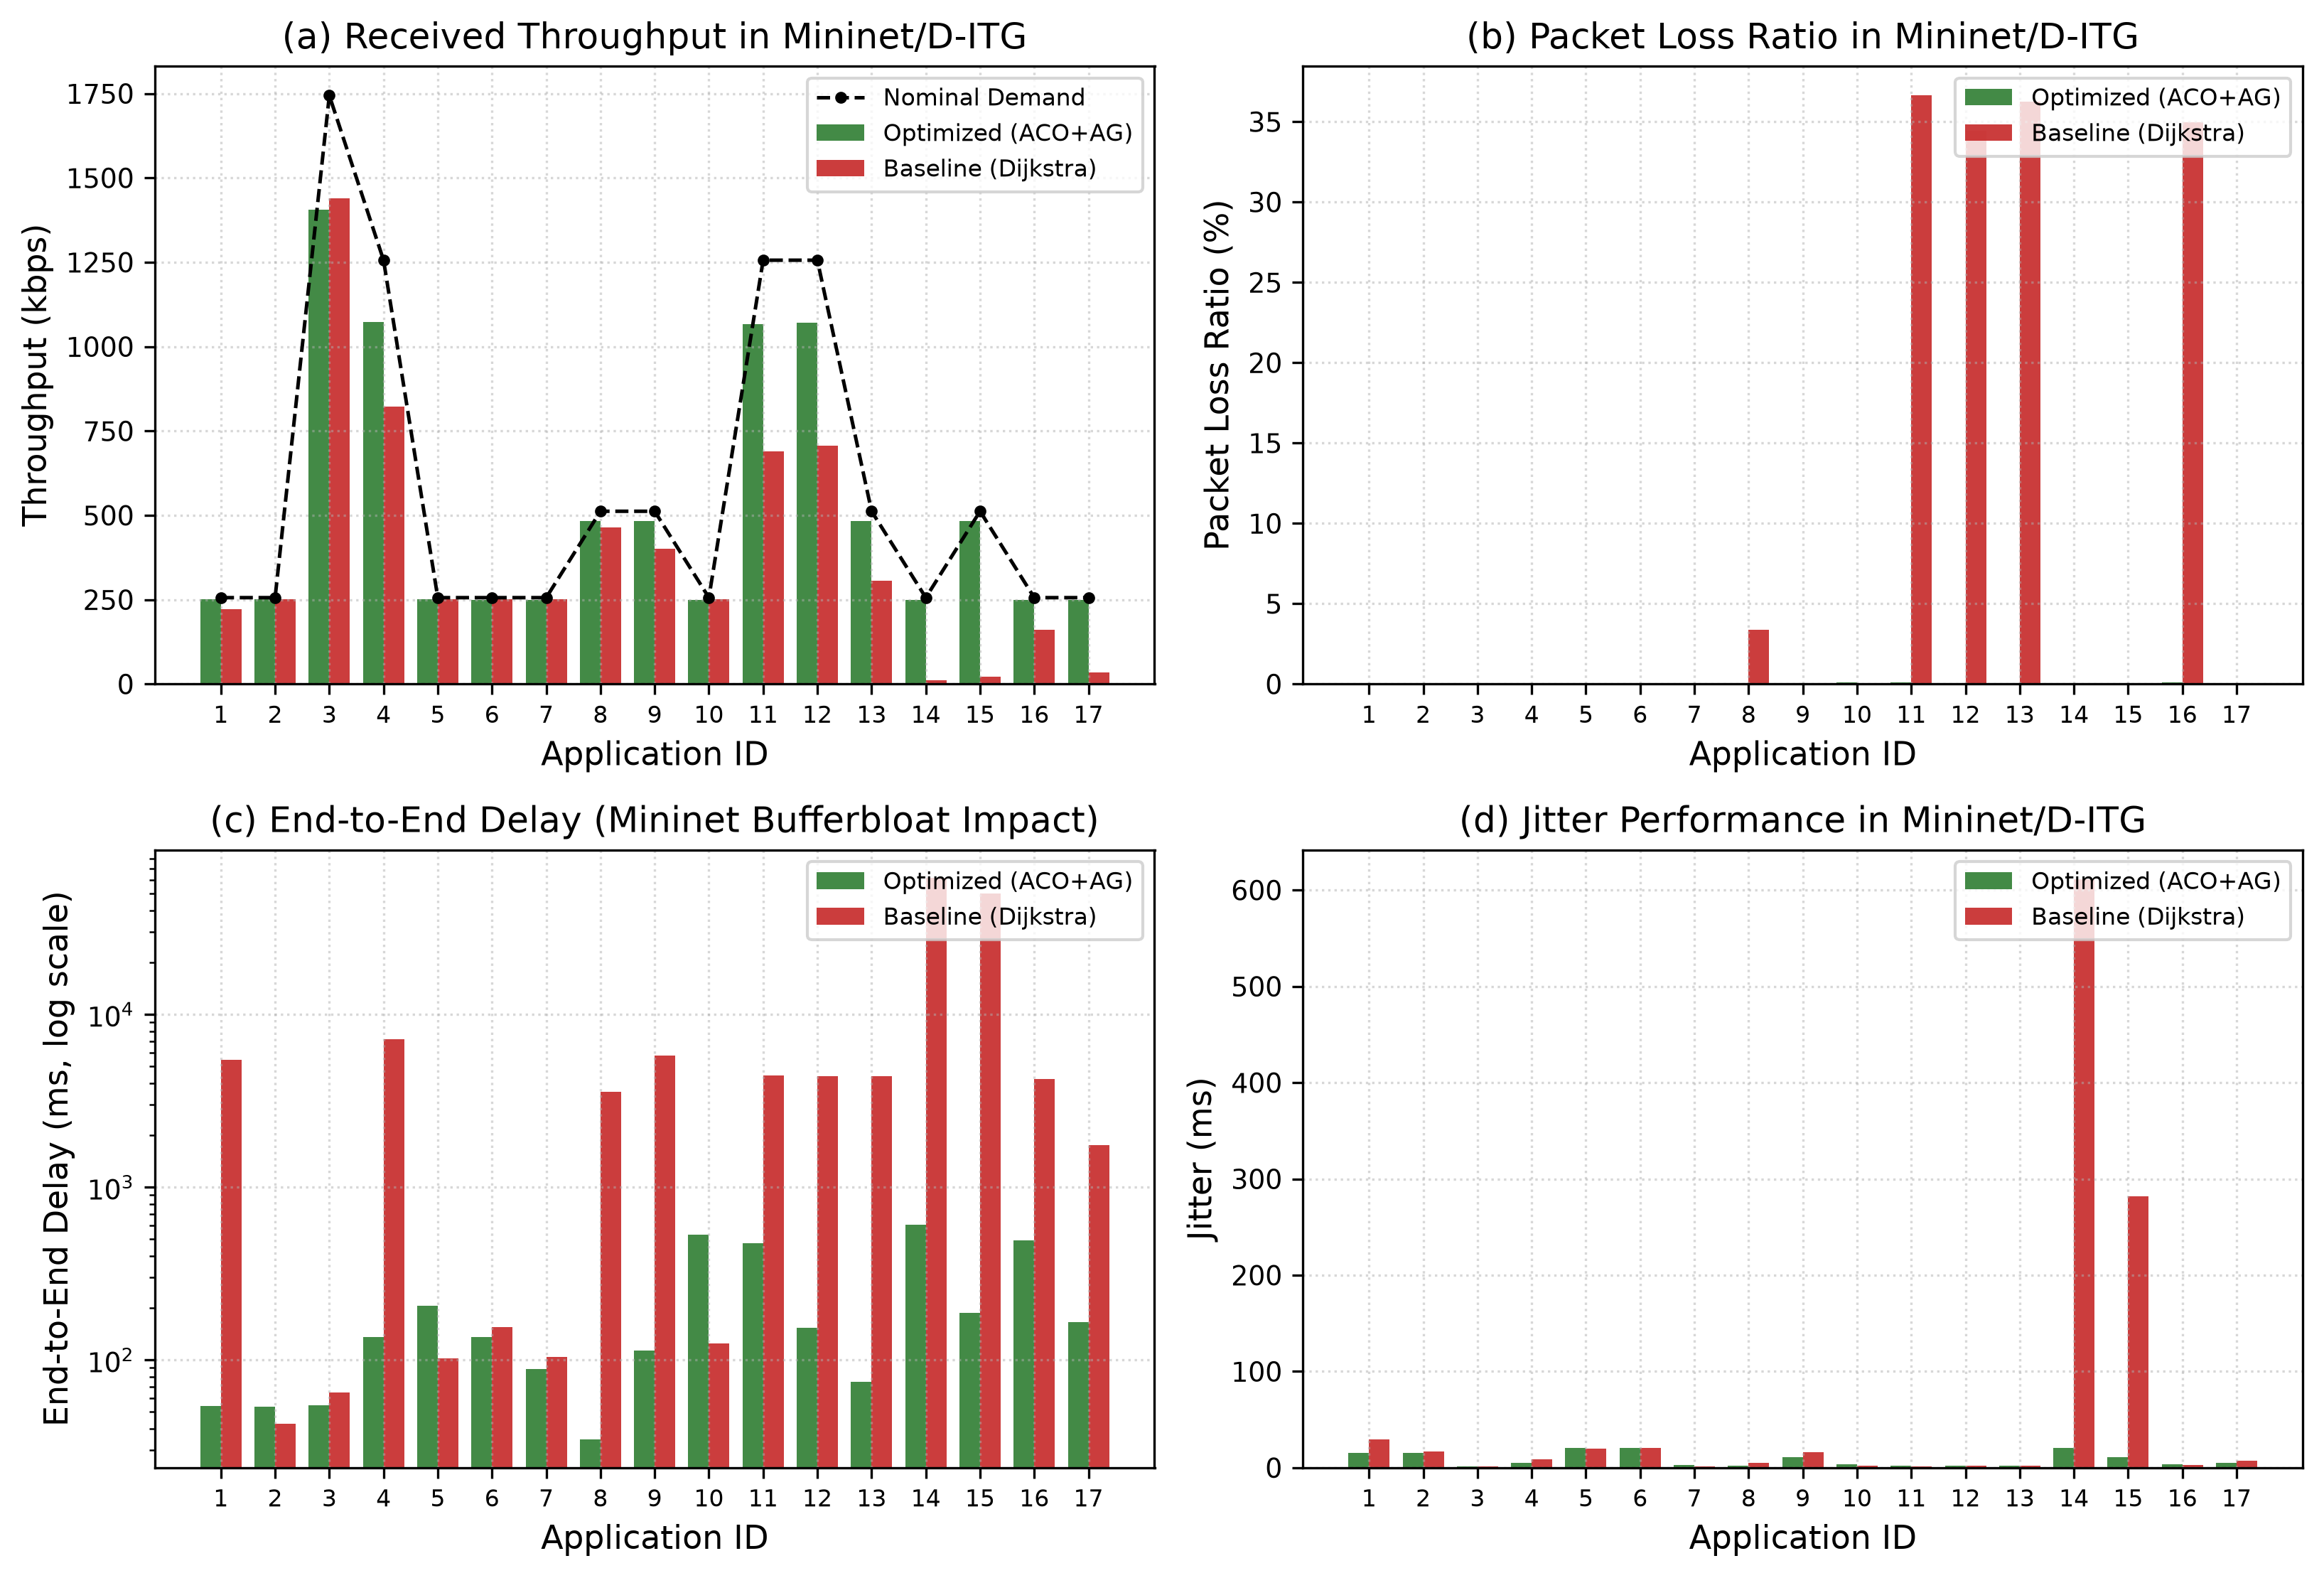
\includegraphics[width=\linewidth]{figures/fig3_mininet_results.png}
\caption{Emulated testbed (Mininet/Floodlight/D-ITG): per-application
throughput, loss, delay and jitter, optimized versus shortest-path routing
(original-study data). The direction of every effect matches the controlled
simulation; magnitudes differ (Section~\ref{sec:bench}).}
\label{fig:mininet}
\end{figure}

\subsection{Logical Differentiation under Background Amplification}
\label{sec:slicesres}
We measure delay-sensitive flows (the four applications mapped to the URLLC
service class in Table~\ref{tab:apps}; 150\,ms is an experimental budget of
this study, not a 3GPP URLLC definition) at nominal rate while the eMBB/mMTC
background is amplified by $1\times$--$4\times$, on both the study instance
and the real German backbone. On \emph{germany50} (Fig.~\ref{fig:slices-ger})
the effect is clean and physically realistic: with optimized routing the
priority flows hold \GerDoptOne\,ms at $1\times$ and \GerDoptTwo\,ms at
$2\times$ with \GerLossOptTwo\% loss, degrading only to \GerDoptThree\,ms at
$3\times$ --- inside the experimental budget --- while shortest-path routing
collapses to \GerDdjTwo\,ms and \GerLossDjTwo\% loss already at
$1.5\times$--$2\times$: the baseline cannot protect the priority flows once
the background grows. On the high-latency study instance \emph{maia52}
(Fig.~\ref{fig:slices}), which is congested even at nominal load, the same
contrast is starker: optimized routing keeps the priority flows at
\UrllcDoptTwo\,ms with loss below \UrllcLossOptTwo\% at $2\times$, whereas
shortest-path routing violates the budget at \emph{every} level
(\UrllcDdjOne\,ms already at $1\times$) and loses up to \UrllcLossDjFour\% at
$4\times$. We deliberately do not call this slice \emph{isolation}: the
capacity constraint is aggregated over all slices on each link and all queues
are FIFO, so what the constraint structure delivers is deterministic,
priority-ordered differentiation under shared capacity --- the priority flows
degrade last and least --- rather than the guaranteed isolation of a
dedicated partition. The real-backbone case shows this mechanism operating
with realistic, sub-2\,ms latencies.

\begin{figure*}[!t]
\centering
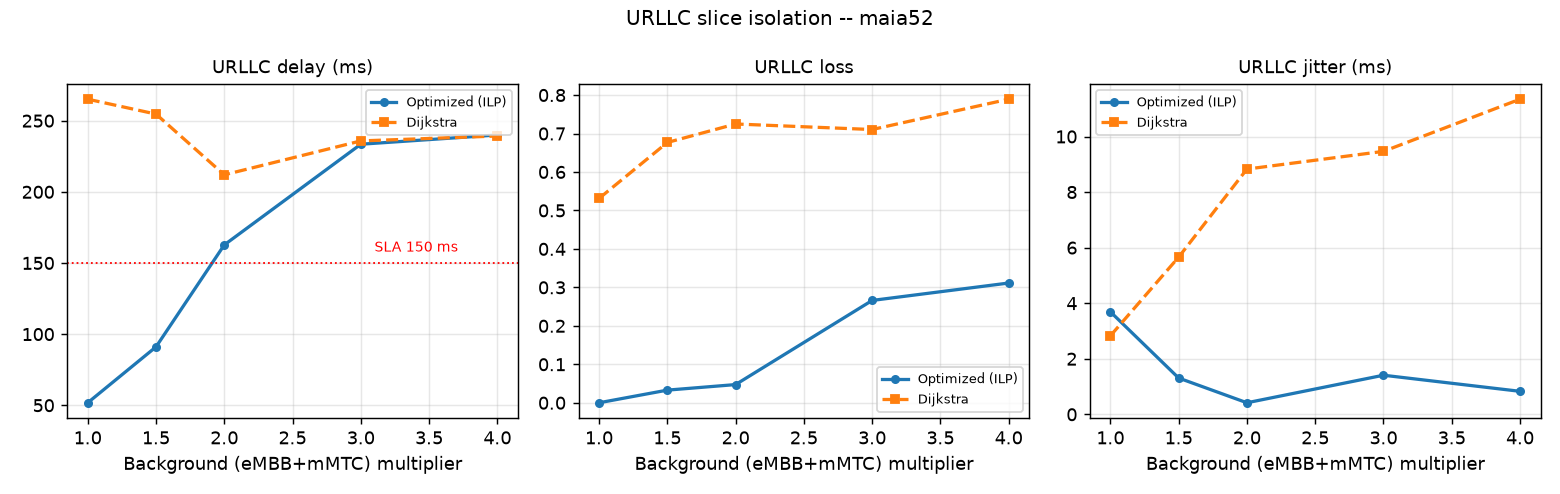
\includegraphics[width=0.92\textwidth]{figures/fig10_slice_isolation.png}
\caption{Delay-sensitive flows (mapped to the URLLC class; 150\,ms
experimental budget) under growing eMBB/mMTC background amplification on the
study instance \emph{maia52}, optimized versus shortest-path routing.}
\label{fig:slices}
\end{figure*}

\begin{figure*}[!t]
\centering
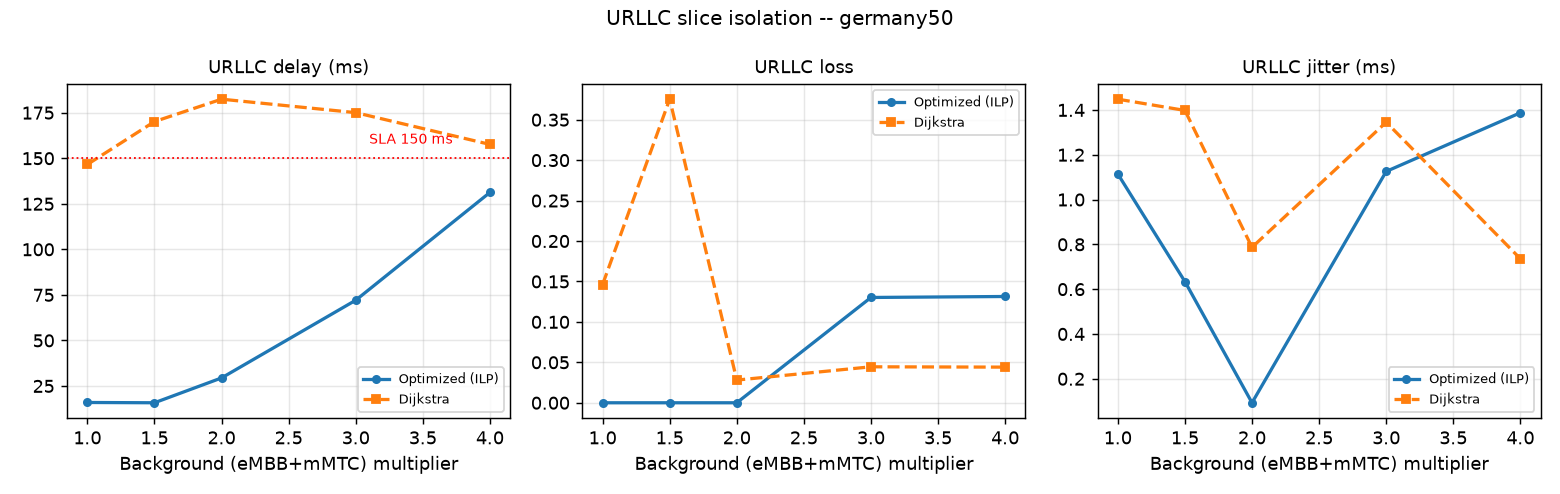
\includegraphics[width=0.92\textwidth]{figures/fig10_germany50_slice_isolation.png}
\caption{Logical differentiation of delay-sensitive flows (URLLC-mapped)
on the \emph{real} German research backbone (\emph{germany50}), with realistic
sub-2\,ms latencies. Optimized routing holds the priority flows at
$\sim\GerDoptTwo$\,ms and $\GerLossOptTwo\%$ loss through $2\times$
background, while shortest-path routing degrades to $\sim\GerDdjTwo$\,ms and
$\GerLossDjTwo\%$ loss from $1.5\times$ onward.}
\label{fig:slices-ger}
\end{figure*}

\subsection{Computed SRv6 State Accounting}
\label{sec:srv6res}
Table~\ref{tab:srv6} and Fig.~\ref{fig:srv6} report the computed data-plane
state (an analytical accounting of rule footprints over the produced paths;
no TCAM measurement or hardware run is claimed). Encoding the same optimized paths as SRv6 segment lists requires
exactly one rule per flow at its headend (\SrvSrRules\ rules for 17 flows)
and \emph{zero} per-flow state at transit nodes, against
\SrvOfMaia--\SrvOfGrid\ per-flow OpenFlow rules distributed over transit
switches across the five instances --- measured reductions of \SrvRedMaia$\times$
(maia52), \SrvRedWax$\times$ (waxman52), \SrvRedGrid$\times$ (gridcore),
\SrvRedGer$\times$ (germany50) and \SrvRedGeant$\times$ (geant2012).
The longest segment list is \MaxSLAll\ SIDs (gridcore) --- which exceeds the
segment-list limits commonly supported by forwarding hardware (typically
6--8 SIDs) and would require uSID/G-SID compression in practice --- yielding
a maximum computed encapsulation overhead of \MaxSrhBytes\ bytes per packet;
denser graphs produce shorter lists (mean \MeanSLWax\ SIDs on waxman52).
Two caveats bound the claim. First, the reduction is computed against the
\emph{worst case} of OpenFlow programming (one rule per flow at every
transit switch); aggregated rules, MPLS labels or tunnels would shrink the
gap. Second, the accounting counts rules, not TCAM bits, programming latency
or SRH forwarding overhead --- the reduction is a state-footprint statement,
not a performance claim. The effect is structural: it holds for every
routing philosophy we computed (Dijkstra, CSPF and the optimizer), because
it moves the path state from the network into the packet.

\begin{figure}[!t]
\centering
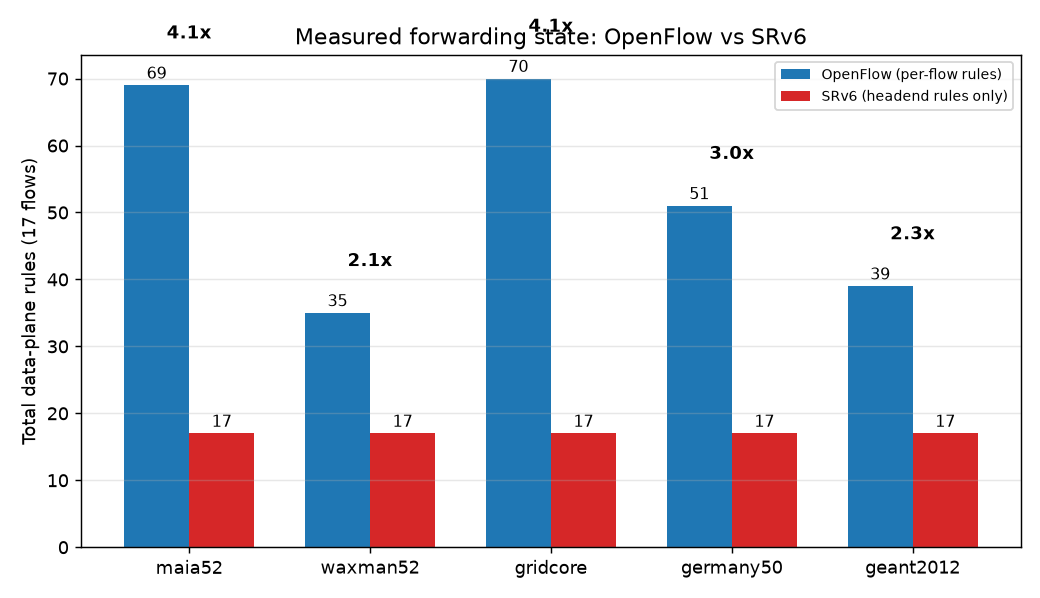
\includegraphics[width=\linewidth]{figures/fig9_srv6_state.png}
\caption{Measured forwarding state for the same 17-flow routing under
per-flow OpenFlow programming versus SRv6 headend-only programming.}
\label{fig:srv6}
\end{figure}

\begin{table}[!t]
\caption{Measured data-plane state (CSPF routing, 17 flows).}
\label{tab:srv6}
\centering
\begin{tabular}{@{}lrrrrr@{}}
\toprule
Topology & OF rules & OF max/node & SRv6 rules & Max SIDs & Reduction\\
\midrule
maia52 & 69 & 9 & 17 & 6 & 4.1$\times$\\
waxman52 & 35 & 4 & 17 & 4 & 2.1$\times$\\
gridcore & 70 & 4 & 17 & 10 & 4.1$\times$\\
germany50 & 51 & 5 & 17 & 6 & 3.0$\times$\\
geant2012 & 39 & 6 & 17 & 8 & 2.3$\times$\\
\bottomrule
\end{tabular}

\end{table}

\subsection{Learning-Based Baseline under the Same Protocol}
\label{sec:qlb}
The tabular Q-learning agent reaches $\QlFOmaia\pm\QlFOmaiaCI$ at nominal
load on maia52 --- near the certified optimum --- but its feasibility is
instance- and seed-sensitive: on the sparse maia52 it assembles a
violation-free route set in only \QlFeasNominal\% of replications at
nominal load, and under stress it inflicts $\QlViolHigh$ violations at
$f=1.25$ versus $\GaViolHigh$ for ACO$+$GA (Wilcoxon $p=\QlVsGaP$), while
on the denser synthetic instances it matches the certified optimum
everywhere. Its per-scenario training ($\QlTime$\,s) is spent again
at every new traffic epoch, whereas the metaheuristic recomputes from the
instantaneous state ($\GaTime$\,s). We state the scope of this evidence
precisely: it concerns \emph{this tabular agent under this protocol}, not
modern DRL routers (GNN-based policies, multi-agent TE), which may close
some of these gaps \cite{xu2018experience,stampa2017drl,almasan2022drl}.
What the experiment does establish is structural: a reward-driven selector
with no constraint model provides no feasibility certificate, and in our
protocol it pays a per-scenario sampling cost. We therefore position
constraint-explicit optimization --- stochastic where scale demands, exact
where affordable --- as the decision core, with learning as an upstream
predictor rather than a replacement.

\subsection{Runtime}
All methods are fast enough for offline TE epochs (Table~\ref{tab:time}):
the exact pool ILP solves in $\PoolTime$\,s, the exact link ILP in
$\IlpTime$\,s, one hybrid run in $\GaTime$\,s, and Q-learning in
$\QlTime$\,s per scenario on a desktop-class CPU --- i.e., optimization
cost is not the operational bottleneck at this scale; certification value is
what distinguishes the methods.

\begin{table}[!t]
\caption{Median wall-clock runtime per complete routing decision (s).}
\label{tab:time}
\centering
\begin{tabular}{@{}lrr@{}}
\toprule
Method & Median runtime (s) & Model\\
\midrule
Dijkstra & 0.0 & deterministic\\
CSPF & 0.0 & deterministic\\
ACO+GA & 6.8 & stochastic\\
ACO+DE & 5.1 & stochastic\\
Q-learning & 0.2 & learning\\
ILP-P (pool) & 0.1 & exact\\
ILP-L (MCF) & 0.6 & exact\\
\bottomrule
\end{tabular}

\end{table}

\subsection{Reconciling Simulation and Emulation}
\label{sec:bench}
The controlled simulation and the emulated testbed agree on the direction of
every effect but differ in magnitude: the bench reports ratios of $51\times$
(delay) and $510\times$ (loss) against shortest-path routing, while the
controlled simulation reports a \SimDelayRatio$\times$ delay ratio and
\emph{elimination} of admission drops (\SimLossOpt\% vs.\ \SimLossDj\%),
which makes the loss \emph{ratio} undefined rather than large. The
explanation is the baseline, not the optimizer: with per-flow
shortest-path routing, a 2\,Mbps bottleneck link carrying several nominal
flows develops a deep persistent queue (bufferbloat; measured 10.8\,s of
queuing delay on the bench). The magnitude of the improvement therefore
depends primarily on queue sizing and queue management of the baseline
deployment --- a configuration artifact --- rather than on the optimizer
itself. We report the controlled simulation with fixed, modest buffers
(80 packets) as the reproducible reference, and the bench as qualitative
confirmation; we explicitly discourage quoting cross-configuration ratios
without stating the queue configuration. The simulator shares one capacity
per undirected link pair between both directions --- the same convention as
the optimizer --- so the combinatorial and packet-level experiments describe
the same network model.

%=====================================================================
\section{Threats to Validity and Limitations}
\label{sec:limits}
\textbf{Scale and link capacity.} The instances span 37--52 nodes and 17--27
flows. Two of them are real backbones, which strengthens external validity but
does not reach carrier or Internet scale. The public GML exports of those
backbones carry no per-link capacity, so --- as stated in
Section~\ref{sec:setup} --- we apply one fixed calibration to place every
instance at the same certified congestion point ($Z^{*}=0.87$ at nominal
load). Absolute capacity values are therefore an experimental control, not a
claim about real provisioned bandwidth; all comparative statements (which
method is feasible, which is better) are invariant to that choice because
every method is evaluated on the identical instance. Heterogeneous,
per-link real capacities remain future work. The ILP formulations scale with
$|E|\,L$ binaries and were solved in seconds here; larger instances would need
decomposition or column generation.
\textbf{Propagation-only delay model.} End-to-end delay in the combinatorial
experiments is propagation plus a fixed per-hop term; queueing delay appears
only in the packet-level simulation. This is why the hard delay constraint is
active on the high-latency synthetic instances and slack on the real
backbones, and it means the capacity constraint --- not the delay budget ---
is the binding one on realistic topologies. Modeling queueing delay inside the
ILP (a stochastic-network extension) is a natural next step.
\textbf{Traffic model.} Constant-rate UDP-style injection abstracts away TCP
dynamics; TCP workloads with congestion control may shift the violation
frontier and are left for future work. The bench evidence (D-ITG) carries
the same abstraction.
\textbf{Load-growth labels.} The factors ``$1.25\times$'' and
``$1.5\times$'' are session-growth parameters; the corresponding aggregate
offered traffic is \LoadRatioHigh$\times$ and \LoadRatioMax$\times$ the
nominal (Section~\ref{sec:setup}). Figures that plot them as a linear
``load factor'' axis should be read with this in mind.
\textbf{Certification tolerance.} The bottleneck bound is certified by a
two-phase lexicographic solve (minimum $Z$, then a delay tie-break with $Z$
pinned to within $10^{-6}$); solves are Optimal for every instance and load
here, but at larger scale the phase-1 time limit would need a stated
optimality gap. At $f\le 1$ the certified bound is dominated by the largest
single flow ($Z^{*}=f\,\lambda_{\max}/\mu$), so its content is the $f>1$
regime (Section~\ref{sec:sweep}).
\textbf{Simulator conventions.} Loss counts admission drops only (in-flight
packets excluded); jitter is the RFC 3550-style mean absolute
consecutive-delay variation, not the D-ITG estimator; capacity is shared per
undirected pair, matching the optimizer. These conventions differ from the
original study's bench and from the earlier draft of this paper; all
packet-level numbers in this version follow them.
\textbf{Pool reuse.} Candidate pools are generated at nominal load and
reused across the sweep; a load-adaptive pool could shift the frontier
slightly, although pool diversity is topology-driven.
\textbf{Objective weights.} The scoring model retains arbitrary weights by
design (continuity with the original formulation); all feasibility and
balancing conclusions are drawn from the revised model, which is
weight-free.
\textbf{Static demands.} The model optimizes a snapshot; reactive
re-optimization under churn and interaction with admission control are open
engineering problems.

%=====================================================================
\section{Conclusion}
\label{sec:conc}
We reformulated QoS-aware traffic engineering for SDN by separating two
models --- the original admission score, which the hybrid optimizes, and a
revised hard-constraint min--max formulation, which we solve exactly and
lexicographically --- and we used the exact solutions to certify, not
assert, the quality of a two-stage hybrid (ACO pool $+$ GA/DE selection) on
five instances (two real backbones), five session-growth factors and twenty
replications. The certificates support four concrete conclusions. The hybrid
attains its certified pool optimum at nominal load on every instance
(17/20 replications on the hardest), and never scores below the constructive
CSPF baseline by construction. The exact model proves where the network's
headroom ends: every routing at $1.25\times$ session growth on the sparse
instance exceeds \IlpZmaiaHighPct\% utilization on some link, while a
feasible routing persists with $1.6\%$ headroom at $1.5\times$ --- yet the
stochastic selector finds it in only \GaFeasMaiaMax\% of replications, a
measurable limit of generate-and-select under stress. On GEANT the
constructive baseline is itself infeasible and the hybrid remains feasible
in \AntGaFeas\% of replications. Packet-level simulation with shared
per-pair capacities shows priority-ordered differentiation --- delay-sensitive
flows degrade last and least --- rather than guaranteed isolation. Finally,
the computed SRv6 accounting bounds the forwarding-state reduction at
$2.1$--$4.1\times$ with transit switches stateless, subject to segment-list
hardware limits. The result is an auditable traffic-engineering core for SDN
controllers: exact where exactness is affordable, heuristic where scale
demands it, and certified everywhere it can be.

\section*{Reproducibility}
All experiments are produced by fixed-seed scripts (topology generation,
ACO pools, metaheuristics, Q-learning baseline, exact ILP models,
packet-level simulation, statistics and figures) released with this paper;
every number in the text is injected from the generated results files.

%=====================================================================
\begin{thebibliography}{30}

\bibitem{mckeown2008} N. McKeown \emph{et al.}, ``OpenFlow: Enabling
innovation in campus networks,'' \emph{ACM SIGCOMM Computer Communication
Review}, vol. 38, no. 2, pp. 69--74, 2008.

\bibitem{kim2013} H. Kim and N. Feamster, ``Improving network management with
software defined networking,'' \emph{IEEE Communications Magazine}, vol. 51,
no. 2, pp. 114--119, 2013.

\bibitem{hu2014} F. Hu, Q. Hao, and M. Bao, ``A survey on software-defined
network and OpenFlow: From concept to implementation,'' \emph{IEEE
Communications Surveys \& Tutorials}, vol. 16, no. 4, pp. 2181--2206, 2014.

\bibitem{bosshart2014} P. Bosshart \emph{et al.}, ``P4: Programming
protocol-independent packet processors,'' \emph{ACM SIGCOMM Computer
Communication Review}, vol. 44, no. 3, pp. 87--95, 2014.

\bibitem{dorigo2004} M. Dorigo and T. St\"utzle, \emph{Ant Colony
Optimization}. MIT Press, 2004.

\bibitem{waxman1988} B. M. Waxman, ``Routing of multipoint connections,''
\emph{IEEE Journal on Selected Areas in Communications}, vol. 6, no. 9,
pp. 1617--1622, 1988.

\bibitem{dicaro1998} G. Di Caro and M. Dorigo, ``AntNet: Distributed
stigmergetic control for communications networks,'' \emph{Journal of
Artificial Intelligence Research}, vol. 9, pp. 317--365, 1998.

\bibitem{awduche2002} D. Awduche \emph{et al.}, ``Overview and principles of
Internet traffic engineering,'' IETF RFC 3272, May 2002.

\bibitem{fortz2000} B. Fortz and M. Thorup, ``Internet traffic engineering by
optimizing OSPF weights,'' in \emph{Proc. IEEE INFOCOM}, 2000,
pp. 519--528.

\bibitem{jain2013} S. Jain \emph{et al.}, ``B4: Experience with a
globally-deployed software defined WAN,'' in \emph{Proc. ACM SIGCOMM},
2013, pp. 3--14.

\bibitem{topozoo} The Internet Topology Zoo: a curated archive of real-world
network topologies, \emph{online}, Jul. 2022. [Online]. Available:
http://www.topology-zoo.org

\bibitem{sndlib2016} S. Orlowski and M. Janiak, ``SNDlib --- a library for
designing multi-instance network design problems,'' Technical Report
TR-11-01, Networks Laboratory, University of Wroc\l aw, Wroc\l aw, Poland,
2011.

\bibitem{xu2018experience} H. Xu, Z. Li, L. Zhou, Z. Li, K. Wang, and Y.
Guo, ``Experience-driven networking: A deep reinforcement learning based
approach,'' in \emph{Proc. IEEE INFOCOM}, 2018, pp. 1871--1879.

\bibitem{stampa2017drl} A. Stampa, M. Arias, D. S\'anchez-Charles, P.
Barlet-Ros, and A. Cabellos-Aparicio, ``A deep-reinforcement learning
approach for software-defined networking routing optimization,'' arXiv
preprint arXiv:1709.07080, 2017.

\bibitem{almasan2022drl} P. Almasan, J. Su\'arez-Varela, A. Badia-Samper, P.
Barlet-Ros, and A. Cabellos-Aparicio, ``Towards deep reinforcement learning
for traffic engineering in SDN,'' \emph{Computer Networks}, vol. 213, art.
109035, 2022.

\bibitem{rfc8402} C. Filsfils, S. Previdi, L. Ginsberg, B. Decraene, S.
Litkowski, and R. Shakir, ``Segment Routing Architecture,'' IETF RFC 8402,
Jul. 2018.

\bibitem{rfc8754} C. Filsfils, D. Dukes, S. Previdi, J. Leddy, S.
Matsushima, and D. Voyer, ``IPv6 Segment Routing Header (SRH),'' IETF RFC
8754, Mar. 2020.

\bibitem{rfc8986} C. Filsfils, P. Camarillo, J. Leddy, D. Voyer, B.
Bernier, and J. Linkova, ``Segment Routing over IPv6 (SRv6) Network
Programming,'' IETF RFC 8986, Feb. 2021.

\bibitem{rfc9256} C. Filsfils, K. Talaulikar, D. Voyer, A. Bogdanov, and P.
Mattes, ``Segment Routing Policy Architecture,'' IETF RFC 9256, Jul. 2022.

\bibitem{rfc4655} A. Farrel, J.-P. Vasseur, and J. Ash, ``A Path Computation
Element (PCE)-Based Architecture,'' IETF RFC 4655, Aug. 2006.

\bibitem{itu-m2083} ITU-R, ``IMT Vision --- Framework and overall objectives
of the future development of IMT for 2020 and beyond,'' Recommendation
ITU-R M.2083-0, Sep. 2015.

\bibitem{3gpp-ts23501} 3GPP, ``System architecture for the 5G System
(5GS),'' Technical Specification TS 23.501, Release 17, 2022.

\bibitem{lantz2010} B. Lantz, B. Heller, and N. McKeown, ``A network in a
laptop: Rapid prototyping for software-defined networks,'' in \emph{Proc.
ACM HotNets}, 2010.

\bibitem{botta2012} A. Botta, A. Dainotti, and A. Pescap\'e, ``On the
validation of D-ITG,'' Technical Report, University of Napoli Federico II,
2012.

\bibitem{watkins1992} C. J. C. H. Watkins and P. Dayan, ``Q-learning,''
\emph{Machine Learning}, vol. 8, pp. 279--292, 1992.

\bibitem{itu2017} International Telecommunication Union, ``ICT facts and
figures 2017,'' Geneva, 2017.

\end{thebibliography}

\end{document}